\scanpage{606}

\deleted{\unsure{To have}} \inserted{The relation} (99),
\deleted{it \unsure{suffices} to \unsure{have}} is written
\[
\tag{102}
\left\{\begin{aligned}
\deleted{\det}\sigma a&\equiv u\quad
(\mathrm{SL}(2,\widehat{\mathbb Z}))\quad\text{i.e.}\quad
\det\sigma a=\det u\quad\text{i.e. (98)}\\
\sigma a&\equiv u\quad(\deleted{4}2)
\end{aligned}\right.
\]
\deleted{\unsure{i.e.}} and this last congruence is written
\[
\tag{103}\begin{gathered}
c\equiv0\quad(\deleted{4}2)\qquad d\equiv1\quad(\deleted{4}2)
\\[3pt]
\left(-d\equiv\mu\quad(\deleted{\unsure{4}}2)\ \text{\unsure{is a consequence of it}}
\ \text{for }\mu\equiv1\equiv-1\quad(2)\right).
\end{gathered}\]

N.B. It is not \unsure{possible to have the} \deleted{\illegible{3} $\mu\equiv-1\ (4)$, for}
congruences \uline{mod 4}
$(\sigma a\equiv u\ (4)$, for we would have
$\mu\unsure{\equiv}-d\equiv-1\ (4)$, which is contrary to the hypothesis
(95) $\mu\equiv1\ (4)$.

\deleted{Thus (102) is \unsure{too strong}. Nevertheless, we \uline{must}
(to have (99)) have
\[
\tag{102 bis}
\sigma a\equiv u\quad(2)\qquad\text{i.e.}
\]
\[
\tag{103 bis}
c\equiv0\quad(2),\qquad d\equiv1\quad(2)
\]
(the relation $-d\equiv\mu\ (2)$ is a consequence of it, for
$\mu\equiv1\equiv-1\ (2)$). \unsure{This}}

Returning to the relation (99), we find this:

\deleted{\uuline{Proposition}} \inserted{Lemma.} Let
$c,d\in\widehat{\mathbb Z}^{\deleted{\unsure{*}}}$ satisfy
\[
\tag{104}
\mu\overset{\mathrm{dfn}}{=}-(c^2+cd+d^2)\in\widehat{\mathbb Z}^{*}
\]
\margin{\uline{N.B.} We will necessaril\textsuperscript{y} have $\mu\equiv-1\ (3)$}
\[
\tag{105}
\mu\equiv1\quad(4)\qquad
(\text{i.e. }c^2+cd+d^2\equiv-1\quad(4)).
\]
\[
\tag{106}
c\equiv0\quad(2),\qquad d\equiv1\quad(2)
\]
Let \deleted{\unsure{a c|a=}} \inserted{\unsure{d}}
\[
\tag{107}
a=\tau'(c\rho+d)=
\begin{pmatrix}-c&c+d\\d&c\end{pmatrix}
\in\mathrm{GL}(2,\widehat{\mathbb Z})
\]
(matrix with determinant $\mu$). Then we have a congruence
\[
\tag{108}
a\tau'(a)^{-1}\equiv\varepsilon\qquad
\mathrm{mod}\ \widehat{\Pi}_0\subset\mathrm{GL}(2,\widehat{\mathbb Z})
\]
\deleted{\unsure{and}} the sign $\varepsilon\in\{\pm1\}$ does not depend on the
choices made for $c,d$.

\scanpage{607}
\mspage{607}

Now is the time to calculate it! Taking up again
\[
a_0=c\rho+d\quad\in Z_\rho
\]
we will have
\[
a=\tau'a_0,\quad \tau'(a)=a_0\tau',\quad
a\tau'(a)^{-1}=\tau'a_0\tau'^{-1}a_0^{-1}=\tau'(a_0)a_0^{-1}
\]
where
\[
\left\{\begin{aligned}
\tau'(a_0)&=c\rho^{-1}+d={}^{t}a_0\\
a_0^{-1}&={}^{t}a_0/\det a_0=-\frac1\mu(c\rho^{-1}+d)
\end{aligned}\right.
\]
\margin{We \unsure{set} \inserted{for
$\unsure{u\in}\mathrm{M}_2(\widehat{\mathbb Z})$}
${}^{t}u=(\mathrm{Tr}\,u)-u$ and we have ${}^{t}\rho=\rho^{-1}$
(more generally ${}^{t}u=u^{-1}$ if $\det u=1$)}
thus
\[
a\tau'(a)^{-1}=\tau'(a_0)a_0^{-1}
=-\frac1\mu(c\rho^{-1}+d)^2
=\frac1{c^2+cd+d^2}(c\rho^{-1}+d)^2
\]
Now we have
\[
(c\rho^{-1}+d)^2
=c^2\underbrace{\rho^{-2}}_{-\rho}
+2cd\underbrace{\rho^{-1}}_{1-\rho}+d^2
=-(c^2+2cd)\rho+(2cd+d^2).
\]
Now \deleted{since}
\[
\begin{aligned}
c\equiv0\quad(2)&\Longrightarrow c^2,2cd\equiv0\quad(4)
\qquad\text{\deleted{thus}}\\
d\equiv1\quad(2)&\Longrightarrow d^2\equiv1\quad(4)
\qquad\text{thus}
\end{aligned}
\]
\deleted{
\[
a\tau'(a)^{-1}\equiv\unsure{\pm}1\quad(4)
\qquad\text{\unsure{a fortiori a}}
\]
}
\[
(\unsure{*})\qquad (c\rho^{-1}+d)^2\equiv1\quad(4)
\]
\deleted{on the other hand.}

\deleted{thus the sign $\varepsilon$ is equal to \uline{$+1$}.}

And since by hypothesis
\[
c^2+cd+d^2\equiv-1\quad(4)
\]
we will have
\[
\tag{109}
a\tau'(a)^{-1}=\frac1{c^2+cd+d^2}(c\rho^{-1}+d)^{\unsure{2}}
\equiv-1\quad(4)
\]
So we have proved, in fact

\uline{Proposition} Let $c,d\in\unsure{\mathbb Z|\widehat{\mathbb Z}}$
be such that $\xi\overset{\mathrm{dfn}}{=}c^2+\unsure{cd}+d^2
\in\widehat{\mathbb Z}^{*}$, let
\[
a=\tau'(c\rho+d)=\begin{pmatrix}-c&c+d\\d&c\end{pmatrix}
\in\mathrm{GL}(2,\widehat{\mathbb Z}),
\]
\deleted{\unsure{let us prove|let us suppose}}
\[
\deleted{(\unsure{110})}\qquad
\deleted{a\tau'(a)^{-1}}\inserted{\sigma a}
\equiv\begin{pmatrix}\xi&0\\0&1\end{pmatrix}
\quad(2)\qquad\text{i.e.}
\]
\figure{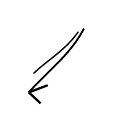
\begin{tikzpicture}[baseline]
\draw[line width=.65pt] (.8,.95) .. controls (.63,.62) and (.36,.43) .. (.1,.14);
\draw[line width=.8pt] (.1,.14)--(.34,.23) (.1,.14)--(.25,0);
\draw[line width=.5pt] (.73,.91) .. controls (.56,.67) and (.35,.56) .. (.16,.38);
\end{tikzpicture}}
\margin{\uline{N.B.} $\sigma=\begin{pmatrix}0&-1\\1&0\end{pmatrix}$}
\[
c\equiv0\quad(2),\qquad d\equiv1\quad(2).
\]

\scanpage{608}

Then we have (for $\tau'=\begin{pmatrix}-1&0\\0&1\end{pmatrix}$)
\[
a\tau'(a)^{-1}\equiv\varepsilon_2(\xi)\quad(4)
\]
(a fortiori we have the congruence mod $\widehat{\Pi}_0$).

\uline{Corollary} The extension $\mathcal E$ of $\mu\times\mu$ by $\mu$
(\unsure{84|89}), or of $\mu$ by $\mathcal E''\simeq\mathbb Z/4\mathbb Z$, is noncommutative.
\margin{$\big|$}

But here is a way of seeing it without calculation. If the extension were commutative,
\deleted{it} \inserted{its isomorphism class} would be given by an
$\unsure{\mathrm{Ext}_{\mathbb Z}|\mathrm{Ext}^1_{\mathbb Z}}$
(or an $\mathrm{Ext}^{\unsure{1|?}}_{\mathbb Z/4\mathbb Z}$).
Now the functor $\unsure{\mathrm{Ext}|\mathrm{Ext}^1}(-,\mu)$ is additive. Since the restriction of
the extension to the subgroups $\mathcal E'/\mu$ and $\mathcal E'''/\mu$ of
$\mu\times\mu$ is trivial, and $\mu\times\mu$ is
the direct sum of these subgroups (which are resp. $1\times\mu$ and the
diagonal subgroup), it would follow that the extension would be
trivial, but we have seen that this is not the case.

\deleted{\unsure{In|And}} \unsure{The} structure of the group $\mathcal E$
is readily made explicit, for example in its \unsure{capacity} as an extension of
$\mathcal E/\mathcal E''\simeq\mu$ by
$\mathcal E''\simeq\mathbb Z/4\mathbb Z$. \deleted{Let}
Let us choose any element of $\mathcal E-\mathcal E''$, it is
of order 2 (the only elements of order 4 being in $\mathcal E''$) so
that we have

\scanpage{609}
\mspage{608}

\[
\tag{110}
\mathcal E\simeq\{1,x\}\mathbin{.}\mathcal E''
\qquad\left(\tfrac12\ \text{direct}\right)
\]
Let us note that if $x$ operated trivially on $\mathcal E''$,
\deleted{i.e.} if $\mathcal E$ were isomorphic to the product, then for an
element \inserted{$u$ of $\mathcal E''$} of order 4,
$x.u$ would be of order \unsure{4|8}, which is absurd (third proof of the fact
that \inserted{$\mathcal E/\mathcal E''\simeq$} $\mu$ operates nontrivially
on $\mathcal E''$). Now from the mere fact that the operation of $\{1,x\}$ on
$\mathcal E''$ is nontrivial\unsure{.}, it is known, and
\inserted{the structure of} $\mathcal E$ is determined -- in fact we have
\[
\tag{\unsure{111|110}}
\mathcal E\simeq\mathbb D_4
\]
There is a preferred choice of $x$, by taking for $x$ the elemen\unsure{t}
\[
\tag{112}
\left\{\begin{aligned}
\tau_{\mathcal E}&\overset{\mathrm{dfn}}{=}
\tau_{\unsure{S_0\Gamma}}\ \mathrm{mod}\ S_0^{\Pi}\Gamma^0,
\quad\text{where of course}\\
\tau_{S_0\Gamma}&=(\tau,\tau',\tau),
\end{aligned}\right.
\]
so that we have a canonical representation
\[
\tag{113}
\mathcal E\simeq\{1,\tau_{\mathcal E}\}\mathbin{.}
\mathcal E''
\qquad\text{product }\tfrac12\text{ direct}
\]
\margin{$\mathcal E''\simeq\mathbb Z/4\mathbb Z$\quad
$\tau_{\mathcal E}(u)=u^{-1}$ for $u\in\mathcal E''$.}

The homomorphism $\mathcal E\to\mu\times\mu$ is recovered from its restrictions to the
two factors
\[
\tag{114}
\diagram{\begin{tikzcd}[column sep=large,row sep=large,column sep=9pt,row sep=14pt,execute at begin picture={\fontsize{10}{12}\selectfont}]
\mu\simeq\{1,\tau_{\mathcal E}\}\arrow[r]&\mu\times\mu&
\tau_{\mathcal E}\arrow[r,mapsto]&(-1,-1)\quad\text{(diagonal homomorphism)}\\
\mathcal E''\arrow[r]&\unsure{\mu\times\{1\}}\arrow[r,hook]&\mu\times\mu&
\end{tikzcd}}
\]
the unique nontrivial homomorphism $\mathcal E''\to\mu$ deduced from the isomorphism
\[
\diagram{\begin{tikzcd}
\mathcal E''_2\overset{\mathrm{dfn}}{=}
\unsure{\mathcal E''/2\mathcal E''|\mathcal E''/{}_{2}\mathcal E''}
\arrow[r,"\sim"]&\mu
\end{tikzcd}}
\]

\scanpage{610}

The fact that $\mathcal E$ is not commutative is also expressed by the fact
that the canonical homomorphism
\[
\tag{115}
\diagram{\begin{tikzcd}
\mathcal E_{\mathrm{ab}}\arrow[r,"\sim"]&\mu\times\mu
\end{tikzcd}}
\]
is an isomorphism, i.e. that the kernel subgroup $\mu$ of
$\unsure{\mathcal E_{\mathrm{ab}}|\mathcal E}\to\mu\times\mu$ is also
the commutator subgroup.

We have seen that the extension $\mathcal E$ of $\mu\times\mu$ by $\mu$ is not
split, but what about its inverse image, the extension
$S_0^{\Pi}\Gamma^!$ of $Z^!\simeq\mathcal M[0]$ by $\mu$? A priori,
we only know that there is no splitting of this extension which
extends the canonical splitting $A$ we have over
\[
Z^0=\mathrm{Ker}\left(\diagram{\begin{tikzcd}
Z^!\arrow[r,"(\varepsilon_3,\varepsilon_2)"]&\mu\times\mu
\end{tikzcd}}\right).
\]
I presume that even $S_0^{\Pi}\Gamma''$, an extension of
$Z^{!\unsure{\prime\prime}}$ by $\mu$, is nontrivial, and
even the extension it induces on the subgroup
\[
\Gamma'_{\mathbb Q}=\Gamma_{\mathbb Q}\cap
\underbrace{\Gamma_{\mathbb Q}^{\prime\sim}}_{\substack{\wr\\\mathcal M(0)'}}
\subset\mathcal M^{\unsure{\xi|*}}(0)\subset\mathcal M^![0]=Z^!.
\]
It would be interesting to identify, \deleted{the ext}
more precisely, the extension over $\Gamma_{\mathbb Q}$, which it induces, which
corresponds to a canonical element
\[
\tag{115}
c\in H^{\unsure{2}}(\mathrm{Spec}\,\mathbb Q,\mu_2)\subset\mathrm{Br}(\mathbb Q)
\]

\scanpage{611}
\mspage{609}

Unless I am mistaken we will have
\[
\tag{115}
c=\underset{\text{(cup-product)}}{\xi'\xi''},
\quad\text{where}\quad
\xi',\xi''\in
H^2(\mathbb Q,\unsure{\mu_2})
\]
are the elements which describe respectively the extensions
$\mathbb Q(\sqrt[3]{1})=\mathbb Q(\sqrt{-3})$, and
$\mathbb Q(\sqrt{3})$ --- both contained, as well as
$\mathbb Q(\sqrt{-1})=\mathbb Q(i)$, in the biquadratic extension
$\mathbb Q\bigl(\underset{\substack{\Vert\\\sqrt[2]{-1}}}{i},
\underset{\substack{\Vert\\\sqrt[3]{1}}}{j}\bigr)
=\mathbb Q(\sqrt[12]{1})$, the field of
$12^{\text{th}}$ roots of unity (whose Galois group is
$(\mathbb Z/12\mathbb Z)^*\simeq(\mathbb Z/3\mathbb Z)^*\times
(\mathbb Z/4\mathbb Z)^*\simeq\mu\times\mu$).

It must be trivial --- when one \unsure{knows} a little of the foundations ---
that $c$ thus made explicit is $\ne0$, and is not
\unsure{split} either on passing to $\mathbb Q(i)$, the third rogue.

\figure{\begin{tikzpicture}\draw (0,0)--(2,0);\end{tikzpicture}}

Let us now consider the central $\mu$-\unsure{grouping}
\margin{\uline{N.B.} $Z\simeq\mathcal M[0]$, $\gamma\simeq\widetilde{\Gamma}_{\mathbb Q}$}
\[
\tag{116}
\diagram{\begin{tikzcd}[column sep=large]
\mu \arrow[r,hook,"i_{\rho,\mu}"] &
S_0\Gamma^!_{\rho,\sigma}
=Z^!_{\rho,\sigma}\times_\gamma N^*_\rho\times_\gamma N^*_\sigma\\
\varepsilon \arrow[r,mapsto] & (1,\varepsilon,1)
\end{tikzcd}}
\]
with values in
\[
\operatorname{Ker}(S_0\Gamma^!_{\rho,\sigma}\longrightarrow
Z^!_{\rho,\sigma})\simeq L_\rho\times L_\sigma,
\]
we thus have a canonical lifting homomorphism
\[
\tag{117}
\diagram{\begin{tikzcd}[column sep=large]
\mathcal M^![0]\simeq Z^!_{\rho,\sigma}
\simeq S_0^\Pi\Gamma^!_{\rho,\sigma}/\mu
\arrow[r] & S_0\Gamma^!_{\rho,\sigma}/i_{\rho,\mu}(\mu),
\end{tikzcd}}
\]

\scanpage{612}

which is made explicit in terms \unsure{\deleted{of the}|of the} two
fundamental canonical homomorphisms
\margin{This deserves to be made explicit in a summarizing theorem $\ldots$}
\[
\tag{118}
\diagram{\begin{tikzcd}[column sep=large,row sep=small]
Z^!_{\rho,\sigma} \arrow[r,"\uline{a}"]
\arrow[d,phantom,"\simeq"{description,sloped}] & N^*_\rho/\mu,
& Z^!_{\rho,\sigma} \arrow[r,"\uline{b}"] & N^*_\sigma\\
\mathcal M[0] \arrow[d,phantom,"\simeq"{description,sloped}] &&&\\
\widetilde{\Gamma}_{\mathbb Q}\mathbin{.}L_0^{\unsure{\Pi}} &&&
\end{tikzcd}}
\]
where, I recall
\[
\tag{119}
\left\{\begin{array}{l}
N^*_\rho\subset\mathcal M=\widetilde N_{1,1}\simeq
\widetilde\Gamma_{\mathbb Q}\mathbin{.}
\underbrace{\mathcal G^+}_{\mathrm{SL}(2,\mathbb Z)^\wedge}\\
\Vert\\
\{u\in\mathcal M\mid
u(\rho)=\deleted{\text{\unsure{fixes the group}}}\rho^{\varepsilon_3(u)}\}\\[1ex]
\deleted{\unsure{\{}}N^*_\sigma\subset\mathcal M\\
\Vert\\
\{u\in\mathcal M\mid u(\sigma)=\sigma^{\varepsilon_2(u)}
\ (=\varepsilon_2(u)\sigma)\}.
\end{array}\right.
\]

The maps $\uline{a},\uline{b}$ are given by the formulas (cf. 51)
\[
\tag{120}
\left\{\begin{array}{ll}
\uline{a}(u)=a=\varepsilon_3[\tau']\alpha^{-1}u,
& \uline{b}(u)=b=\beta^{-1}u\quad\text{i.e.}\\
\alpha=ua^{-1}\varepsilon_3[\tau'],&\beta=ub^{-1}
\end{array}\right.
\]
where $\alpha\in\widehat\Pi_{0\tau}$, $\beta\in\widehat\Pi_0$
are characterized by
\[
\tag{121}
u(\rho)=\operatorname{int}(\alpha)(\rho),\quad
u(\sigma)=\varepsilon_2(\sigma)\operatorname{int}(\beta)(\sigma).
\]
The quantities \deleted{\unsure{$a,$}}
$a=\uline{a}(u)\inserted{\in N^*_\rho/\mu}$,
$b=\uline{b}(u)\inserted{\in N^*_\sigma}$ are characterized in terms of
$u\in Z^!$ (only up to a sign) by the congruences
\[
\tag{122}
u\equiv b\quad(\widehat\Pi_0),\qquad
u\equiv\varepsilon_3[\sigma]a\quad(\widehat\Pi),
\]
which imply a fortiori (reducing mod $\mathcal G^{+\wedge}$),
that we have commutativity \unsure{of the|of},

\scanpage{613}
\mspage{\unsure{619|610}}

\deleted{(\unsure{123|122})}
\[
\tag{123}
\diagram{\begin{tikzcd}[column sep=large,row sep=small]
&N^*_\rho/\{\unsure{\pm}1\}\arrow[dr,"\delta_\rho"]&\\
Z^!_{\rho,\sigma}\arrow[ur]\arrow[dr]
\arrow[rr,dashed,"\delta_Z"]&&\gamma_{\rho,\sigma}\simeq\widetilde\Gamma_{\mathbb Q}\\
&N^*_\sigma\arrow[ur,"\delta_\sigma"']&
\end{tikzcd}}
\]

\deleted{Let us now consider the two $\mu$-groupings}
\[
\deleted{(124)}\qquad
\diagram{\begin{tikzcd}[column sep=large,nodes in empty cells]
\deleted{\mu}\arrow[r] &
\deleted{S_0\unsure{\mathcal M|\Gamma}_{\rho,\sigma}}
\end{tikzcd}}
\]

It would be time to rectify the confusion (page\ \unsure{594'}) between
$Z=Z_{\rho,\sigma}\not\subset
\mathcal M_{0,3}^{\unsure{\circ|\bullet}\sim}$,
and $Z^!=Z^!_{\rho,\sigma}=\deleted{\unsure{\mathcal M}}
Z\cap\mathcal M_{0,3}^{!\sim}$.
We have in fact
\[
\tag{124}
\diagram{\begin{tikzcd}[column sep=small,row sep=large]
Z_{\rho,\sigma}^{\deleted{\unsure{!}}}\simeq
\underset{\frac12\text{-direct}}{\mathcal M^{\unsure{\xi}}(0)\mathbin{.}L_0^{\mathcal G}}
\subset\mathcal M\arrow[dr,"\sim"]&\\
&\mathcal M_{0,3}^{\unsure{\xi}\sim}(0)\mathbin{.}
L_0^{\mathcal G_{0,3}}\subset\widetilde{\mathcal M}_{0,3}
\end{tikzcd}}
\]
\[
\tag{125}
\diagram{\begin{tikzcd}[column sep=small,row sep=large]
Z^!_{\rho,\sigma}\simeq Z^!_{\rho,\sigma}\cap\mathcal M^!
=\underset{\frac12\text{-direct}}{\mathcal M(0)\mathbin{.}L_0^\Pi}
\subset\mathcal M\arrow[dr,"\sim"]&\\
&\widetilde{\mathcal M}_{0,3}(0)\mathbin{.}L_0^{\Pi_{0,3}}
\deleted{\unsure{\subset\widetilde{\mathcal M}_{0,3}}}
\inserted{(\subset\widetilde{\mathcal M}_{0,3})}
\end{tikzcd}}
\]

The link between the two is given by the diagram
\[
\tag{126}
\diagram{\begin{tikzcd}[column sep=small,row sep=large]
1\arrow[r]&L_0^\Pi\arrow[r]\arrow[d,hook]&
Z^!_{\rho,\sigma}\arrow[r]\arrow[d,hook]&
\gamma_{\rho,\sigma}\arrow[r]\arrow[d,equal]&1\\
1\arrow[r]&L_0^{\mathcal G}\arrow[r]&
Z_{\rho,\sigma}\arrow[r]&
\gamma_{\rho,\sigma}\arrow[r]
\arrow[d,phantom,"\simeq"{description,sloped}]&1\\
&&&\mathcal M(0)\simeq\widetilde\Gamma_{\mathbb Q}&
\end{tikzcd}}
\]
where $L_0^\Pi\longrightarrow L_0^{\mathcal G}$ is
the inclusion of index $2$ of
\[
\tag{127}
\diagram{\begin{tikzcd}[column sep=large,row sep=small]
L_0^\Pi=\ell_0^{\widehat{\mathbb Z}}
\arrow[r,hook]\arrow[d,phantom,"="{description,sloped}]&
\deleted{\unsure{\ell_0^{\widehat{\mathbb Z}}|\varepsilon_0^{\widehat{\mathbb Z}}}}
L_0^{\mathcal G}=\varepsilon_0^{\widehat{\mathbb Z}}\\
\varepsilon_0^{2\widehat{\mathbb Z}}&
\end{tikzcd}}
\]
Of course, it is indeed on $Z^!_{\rho,\sigma}$, not on
$Z_{\rho,\sigma}$, that we defined (117), (118) whence (123).

\scanpage{614}

I am interested in the restriction of the homomorphisms (123) to the subgroup
$L_0^\Pi$ of $Z^!_{\rho,\sigma}$
the characterization (122) shows that the induced homomorphism
\[
\diagram{\begin{tikzcd}[column sep=large]
L_0^\Pi\arrow[r]&N^*_\rho/\{\pm1\}
\end{tikzcd}}
\]
\deleted{is}
is trivial (for $a$ in terms of $u$ depends only on $u$ modulo
$\widehat\Pi$), whereas the induced homomorphism
\[
\diagram{\begin{tikzcd}[column sep=large]
L_0^\Pi\arrow[r]&N^*_\sigma
\end{tikzcd}}
\]
factors through $L_0^\Pi/L_0^{\Pi_0}\simeq\mathbb Z/2\mathbb Z$
(for $b$ in terms of $u$ depends only on $u$ modulo $\widehat\Pi_0$).
Its value \inserted{$b$} on \deleted{$\varepsilon_0$} $\ell_0$ is
\deleted{given}\inserted{\unsure{characterized|characterized}}
by the conditions
\[
\unsure{\{}\qquad b\in N^*_\sigma,\qquad b\equiv\ell_0\quad(\Pi_0)
\]
which are obviously satisfied by $b=-1$. Thus
There is reason to introduce also, whether we like it or not, the
canonical central $\mu$-grouping
\[
\tag{128}
\diagram{\begin{tikzcd}[column sep=large]
\mu\arrow[r,hook]&N^*_\sigma\\
-1\arrow[r,mapsto]&-1
\end{tikzcd}}
\]
and we have commutativity of
\[
\tag{129}
\diagram{\begin{tikzcd}[column sep=large,row sep=large]
L_0^\Pi\arrow[r,hook]\arrow[d]&Z^!_{\rho,\sigma}\arrow[d]\\
L_0^\Pi/L_0^{\Pi_0}\simeq\mu\arrow[r,hook]&N^*_\sigma.
\end{tikzcd}}
\]
Thus we find, from the two homomorphisms (123),

\scanpage{615}
\mspage{611}

of $Z^!_{\rho,\sigma}$, by passage to the quotient two canonical homomorphisms
\[
\tag{130}
\left\{
\diagram{\begin{tikzcd}[column sep=large,row sep=small]
\gamma_{\rho,\sigma}\arrow[r]\arrow[d,equal]&N^*_\rho/\{\pm1\}\\
\widetilde\Gamma_{\mathbb Q}\arrow[d,equal]&\\
\gamma_{\rho,\sigma}\arrow[r]&N^*_\sigma/\{\pm1\},
\end{tikzcd}}
\right.
\]
which are in fact sections of the
\[
\diagram{\begin{tikzcd}[column sep=large,row sep=small]
N^*_\rho/\{\pm1\}\arrow[r]&\gamma_{\rho,\sigma}\arrow[d,equal]&\\
&\widetilde\Gamma_{\mathbb Q}\arrow[d,equal]&\mathcal M(0)\arrow[l,"\sim"']\\
N^*_\sigma/\{\pm1\}\arrow[r]&\gamma_{\rho,\sigma},&
\end{tikzcd}}
\]
so that we find decompositions,
\[
\tag{131}
\left\{\begin{array}{l}
N^*_\rho/\pm1\simeq\gamma_{\rho,\sigma}
\deleted{\unsure{\ltimes|\times}}\mathbin{.}
\underbrace{SZ_\rho/\{\pm1\}}_{=L_\rho/\{\pm1\}\simeq\mathbb Z/3\mathbb Z}\\[2ex]
N^*_\sigma/\pm1\simeq\gamma_{\rho,\sigma}\mathbin{.}
\underbrace{SZ_\sigma/\pm1}_{=L_\sigma/\pm\ \simeq\mathbb Z/2\mathbb Z}
\end{array}\right.
\]
($\frac12$-direct products). The operation of $\gamma_{\rho,\sigma}$ on
$L_\rho/\{\pm1\}\simeq\mathbb Z/3\mathbb Z$ is given by the
quadratic character $\varepsilon_3$, the one on
$L_\sigma/\{\pm1\}\simeq\mathbb Z/2\mathbb Z$ is given by the quadratic
character $\varepsilon_2$.

The symmetry of presentation of the two homomorphisms (130) is a bit
\unsure{phony} --- for example the homomorphism
$\widetilde\Gamma_{\mathbb Q}=\gamma_{\rho,\sigma}\longrightarrow
N^*_\sigma/\{\pm1\}$ lifts in an obvious way to
\[
\tag{132}
\diagram{\begin{tikzcd}[column sep=small,row sep=large]
\widetilde\Gamma_{\mathbb Q}=\gamma_{\rho,\sigma}\arrow[rr]&&N^*_\sigma,&\\
&\mathcal M(0)\arrow[ul,"\sim"]
\arrow[rr,phantom,"\subset"{description}]&&\mathcal M[0]=Z^!\arrow[ul]
\end{tikzcd}}
\]

\scanpage{616}

Another way to see this is to note that
\[
 (132)\qquad \gamma_{\rho,\sigma}\simeq
 \mathcal M_0^{\unsure{!}}[0]/L_0^{\Pi_0}
\]
where
\[
 \mathcal M_0^{\deleted{\unsure{*}}!}[0]
 \overset{\mathrm{dfn}}{=}
 \mathcal M_{\unsure{\delta|0}}(0).L_0^{\Pi_0}
 \underset{\substack{\text{subgroup}\\\text{of index }2}}{\subset}
 \mathcal M^![0]=\mathcal M(0).L_0^{\unsure{\Pi|\tau}}
\]

Now on $L_0^{\Pi_0}$, the homomorphism induced by
\diagram{\begin{tikzcd}
 \mathcal M^![0]=Z^!_{\rho,\sigma} \arrow[r] & N^*_{\sigma}
\end{tikzcd}}
is trivial. Thus we even have a
\deleted{\unsure{isomorphism}} splitting of
\[
 (133)\qquad
 \diagram{\begin{tikzcd}[column sep=large]
 1 \arrow[r] & L_{\sigma} \arrow[r] & N^*_{\sigma} \arrow[r]
 & \gamma_{\rho,\sigma} \arrow[r] \arrow[d, phantom, "\simeq" {rotate=90}] & 1\\
 &&& \widetilde{\Gamma}_{\mathbb Q}
 \end{tikzcd}}
\]
as a $\frac12$-direct product
\[
 \deleted{\unsure{(134)}}\qquad
 N^*_{\sigma}\simeq\gamma_{\rho,\sigma}.L_{\sigma}
\]
which it is better to write by concretizing the section subgroup \unsure{as}
a subgroup of $G_{\rho,\sigma}\simeq\mathcal M$, i.e. then
\[
\begin{aligned}
 (134)\qquad
 \unsure{N}_{0\sigma}^{!*}
 &\overset{\mathrm{dfn}}{=}
 \operatorname{Im}(\mathcal M_0[0]\longrightarrow N^*_{\rho})\\
 &=\operatorname{Im}(\mathcal M[0]\hookrightarrow N^*_{\rho})\\
 &=\{\beta^{-1}u\mid u\in\mathcal M(0),\ \beta\in\widehat\Pi_0
       \text{ such that }u(\sigma)=\varepsilon_{\unsure{2}}(u)
       \operatorname{int}(\beta)(\sigma)\}\\
 &=\{v\in N^*_{\sigma}\mid \exists\,\beta\in\widehat\Pi_0\text{ such that }
       \beta v\in\mathcal M[0]=\operatorname{Norm}_{\mathcal M}(\unsure{l_0})
       \cap\mathcal M^!\}
\end{aligned}
\]
\margin{\uline{N.B.} We define $\mathcal M^!$ as the inverse image of
$\mathcal M_{0,3}^{!\sim}$, i.e. the kernel of the canonical representation
\diagram{\begin{tikzcd}
 \mathcal M \arrow[r] &
 \underbrace{\mathcal G^{+\wedge}/\Pi^{\wedge}}_{\mathcal G_3}
 \arrow[r,"\sim"] &
 \operatorname{Aut}(\mathcal G^{+\wedge}/\Pi^{\wedge})
\end{tikzcd}}}

Setting
\[
 (135)\qquad
 \mathcal M_0^!\overset{\mathrm{dfn}}{=}\mathcal M(0).\Pi_0
 \underset{\substack{\text{index}\\2}}{\subset}
 \mathcal M^!\overset{\mathrm{dfn}}{=}\mathcal M(0).\Pi,
\]

\scanpage{617}
\mspage{612}

so that we have
\[
 (136)\qquad \mathcal M^!\simeq\mathcal M_0^!\times\mu,
\]
\margin{\uline{N.B.} We have
\diagram{\begin{tikzcd}
 \mathcal M_0^!\arrow[r,"\sim"] & \mathcal M_{0,3}^{!\sim}
\end{tikzcd}}}
we thus have
\[
 (137)\qquad
 \left\{\begin{aligned}
 N_{\sigma0}^{\deleted{\unsure{d}}*!}&=N^*_{\sigma}\cap\mathcal M_0^!\\
 N_{\sigma}^{*!}&\overset{\mathrm{dfn}}{=}N^*_{\sigma}\cap\mathcal M^!
                    =N_{\sigma0}^{*!}\times\mu,
 \end{aligned}\right.
\]
and we find that
\[
 (138)\qquad
 \diagram{\begin{tikzcd}
 N_{\sigma0}^{\unsure{*!|d!}}\arrow[r,"\sim"] &
 \gamma_{\rho,\sigma}=\widetilde\Gamma_{\mathbb Q}
 \end{tikzcd}}
\]
\deleted{\unsure{whence}} Let us set for short
\[
 \deleted{(139)\qquad N_{\sigma}^{\unsure{d}}\simeq N_{\sigma0}^{*!}}
\]
\[
 (139)\qquad \mathcal M(1/2)=N_{\sigma0}^{*!}\qquad\text{cf. }(137)
\]
we will thus have that $\mathcal M(1/2)$ is \unsure{a|a}
\inserted{\unsure{group-}}section
\deleted{(140)} for $N_{\sigma}^{\unsure{*|\wedge}}$ extension of
$\gamma_{\rho,\sigma}$ by $L_{\unsure{\sigma|\rho}}$, and a fortiori for
$\mathcal M$ extension of $\gamma_{\rho,\sigma}$ by $\mathcal G^{+\wedge}$,
and \unsure{one|we} \unsure{even|\simeq} \unsure{in addition|simple} for
$\mathcal M_0^!,\mathcal M^!$
\[
 (140)\qquad
 \left\{\begin{aligned}
 \mathcal M_0^!&\simeq\mathcal M(1/2).\widehat\Pi_0\\
 \mathcal M^!&\simeq\mathcal M(1/2).\widehat\Pi\\
 \mathcal M&\simeq\mathcal M(1/2).\mathcal G^{+\wedge}\\
 N^*_{\sigma}&\simeq\mathcal M(1/2).L_{\sigma}
 \end{aligned}\right.
\]
\margin{$\longleftarrow$ watch out, $\mathcal M^!$ is inverse in $\mathcal M$
and $\mathcal M_0^!$ is inverse in $\mathcal M^!$, but
\uline{not in} $\mathcal M$\quad cf. below}

[If we want to \unsure{paraphrase} by introducing
\[
 (141)\qquad
 N_{\rho0}^{*!}\overset{\mathrm{dfn}}{=}N^*_{\rho}\cap\mathcal M_0^!
 =\{v\in N^*_{\rho}\mid\exists\,\alpha\in\widehat\Pi_0\text{ such that }
       \underbrace{\alpha v}_{u}\in\mathcal M(0)\}
\]
it is thus one of the $v$ that we can associate to the
$u\in\mathcal M(0)\subset\mathcal M^![0]=Z^!_{\rho,\sigma}$,
using the $\alpha\in\Pi_0$ such that
$\alpha^{-1}u\in N_{\rho}^{\unsure{*|\wedge}}$ i.e.
\[
 u(\rho)=\operatorname{int}(\alpha)(\rho^{\varepsilon_3})
 \qquad\text{where}\quad\varepsilon_3=\varepsilon_3(u)=\varepsilon_3(v).
\]
But since $u(\rho)$ must have the same image in
$\mathcal G_3=\mathcal G^{+\wedge}/\Pi$
as $\rho$, we must have $\varepsilon_3=1$, and then
$\alpha$ is the element $\uline{\alpha}(u)$ associated to $u$ and
$v=\alpha^{-1}u$ is the canonical image of $u$ in $N^{!*}_{\rho}$. Thus we

\scanpage{618}

find

\uline{Proposition} The homomorphism
$N_{\rho0}^{*!}\longrightarrow\gamma_{\rho,\sigma}=\widetilde\Gamma_{\mathbb Q}$
is injective, and has image
$\gamma'_{\rho,\sigma}=\{\gamma\in\gamma_{\rho,\sigma}\mid\varepsilon_3(\gamma)=1\}$.

\uline{Corollary}
$N_{\rho,0}^{*!}\subset Z_{\rho}^{\unsure{\xi|*}!}$ i.e.
$N_{\rho0}^{*!}=\deleted{\unsure{N}}Z_{\unsure{0\rho|\rho0}}^{\unsure{\xi|*}!}
 \overset{\mathrm{dfn}}{=}Z_{\rho}^{\unsure{\xi|*}}\cap\mathcal M_0^!$.

It is natural to set
\[
 (142)\qquad N_{\rho0}^{*!}=Z_{\rho0}^!=\mathcal M(-\bar j)\,\unsure{..|.}
\]
Since $N_{\rho}^{*!}\supset Z_{\rho}^!\supset\mu$, we see that we have
\[
 (142)\qquad
 \left\{\begin{array}{rcll}
 N_{\rho\deleted{\unsure{0}}}^{*!}&=&N_{\rho0}^{*!}\times\mu
     &\bigl(\text{thus }N_{\rho}^{*!}=Z_{\rho}^!\bigr)\\
 \Vert&&&\\[-1ex]
 Z_{\rho}^!&=&Z_{\rho\unsure{0}}^!\times\mu&
 \end{array}\right.
\]
\[
 \deleted{\unsure{N_{\rho}}\simeq}
\]

The subgroup $Z^!_{0,\rho}=\mathcal M(-\bar j)$ is a section of
$\mathcal M'$ over $\gamma'_{\rho,\sigma}\simeq\Gamma_{\mathbb Q}^{\prime\sim}$,
and \deleted{\unsure{is}} \inserted{\unsure{$\mathcal M'$}}
\unsure{contained|contained} in
\deleted{$Z^!_{0\rho}$ a fortiori in}
$\mathcal M_0^{\prime!},\mathcal M^{\prime!},
 \deleted{\unsure{Z_{0\rho}}},Z_{\rho}^!,Z_{\rho}$,
we will have decompositions into $\frac12$ direct products
\[
 (143)\qquad
 \left\{\begin{aligned}
 \mathcal M_0^{\prime!}&\simeq\mathcal M(-\bar j).\Pi_0\\
 \mathcal M^{\prime!}&\simeq\mathcal M(-\bar j).\Pi\\
 \mathcal M^{\prime\unsure{\xi|*}}&\simeq\mathcal M(-\bar j).\mathcal G\\
 Z_{\rho}^!&\simeq\deleted{Z}\mathcal M^{\unsure{\xi|*}}(-\bar j)\times\mu\\
 Z_{\rho}^{\unsure{\xi|*}}&\simeq\mathcal M^{\unsure{\xi|*}}(-\bar j)\times L_{\rho}
 \qquad ....
 \end{aligned}\right.
\]
]

\deleted{Let us now note that}
\[
 \deleted{\mu_{\tau'}\overset{\mathrm{dfn}}{=}\{1,\tau'\}\subset\mathcal G^{\wedge}}
\]
\deleted{normalizes $L_{\rho}$, hence $Z_{\rho}$, hence
$Z^!_{0,\rho}=Z_{\rho}\cap\mathcal M_0^!$}

\scanpage{619}
\mspage{613}

Let us return to diagram (130), I say that the homomorphism
\diagram{\begin{tikzcd}
 \gamma_{\rho,\sigma}\arrow[r]\arrow[d,phantom,"\Vert"] & N^*_{\rho}/\{\pm1\}\\
 \Gamma_{\mathbb Q}^{\sim}
\end{tikzcd}}
\uline{does not lift} to a homomorphism from $\gamma_{\rho,\sigma}$ to
$\underset{\inserted{\widetilde\gamma_{\rho,\sigma}}}{N^*_{\rho}}$
--- in other words, that the extension of $\gamma_{\rho,\sigma}$ by
$\{\pm1\}=\mu$ which it defines is not trivial. To identify this
extension, let us consider the diagram
\margin{\uline{N.B.}}
\[
(144)\qquad
\diagram{\begin{tikzcd}[column sep=large,row sep=huge,column sep=9pt,row sep=14pt,execute at begin picture={\fontsize{10}{12}\selectfont}]
 \mathcal M^![0]=Z^!_{\rho,\sigma}\arrow[rr,"\text{canonical}"]
 &&\gamma_{\rho,\sigma}=Z^!_{\rho,\sigma}/L_0^{\Pi}
       \arrow[r,"\text{homomorphism }(130)"]
 &[60pt]N^*_{\rho}/\{\pm1\}\\
 S_0\Gamma^!_{\rho,\sigma}
       \arrow[u,"{\text{canonical}\quad(u,a,b)\mapsto u}"']
 &\inserted{\unsure{S_0}\Gamma_{\rho,\sigma}\quad\text{(without !)}}
       \arrow[ur,very thick,"{\substack{\text{canonical}\\\unsure{\text{(passage to the quotient)}}}}"']
 &&\\
 S_0^{\Pi}\Gamma^!_{\rho,\sigma}\arrow[u,hook,"\text{inclusion}"']
       \arrow[ur,hook,dashed,"\text{inclusion}"']\arrow[rrr]
 &&&N^*_{\rho}\arrow[uu]
\end{tikzcd}}
\]
which shows that we have a diagram of cartesian squares
\[
(145)\quad\deleted{\unsure{(146)|(144)}}\qquad
\diagram{\begin{tikzcd}[column sep=large,row sep=huge]
 \mathcal M(0)\arrow[r,hook]\arrow[dr,phantom,"\mathrm I" description]
 &\mathcal M^![0]=Z^!_{\rho,\sigma}\arrow[r,"\text{epimorphism}"]
       \arrow[dr,phantom,"\mathrm {II}" description]
 &\gamma_{\rho,\sigma}\arrow[r,hook]
       \arrow[dr,phantom,"\mathrm {III}" description]
 &N^*_{\rho}/\{\pm1\}\\
 \mathcal M(0)^{\sim}\arrow[u]\arrow[r,hook]
 &S_0^{\Pi}\Gamma^!_{\rho,\sigma}\arrow[u,"2"]\arrow[r]
 &\widetilde\gamma_{\rho,\sigma}\arrow[u,"2"]\arrow[r,hook]
 &N_{\rho}^{\unsure{*|d}}\arrow[u,"2"]
\end{tikzcd}}
\]
where $\mathcal M(0)^{\sim}$ is \unsure{defined|defined} as the extension of
$\mathcal M(0)$ by $\mu$ induced by the extension
$S_0^{\Pi}\Gamma^!_{\rho,\sigma}$ of $\mathcal M^![0]$,
which is thus identified \unsure{also} with the \unsure{inverse|inverse} image of

\scanpage{620}

the extension $\widetilde\gamma_{\rho,\sigma}$ of $\gamma_{\rho,\sigma}$ by $\mu$,
under the composite isomorphism
\diagram{\begin{tikzcd}
 \mathcal M(0)\arrow[r,"\sim"] & \gamma_{\rho,\sigma}.
\end{tikzcd}}
So the extension $\widetilde\gamma_{\rho,\sigma}$ of $\gamma_{\rho,\sigma}$ by
$\mu$ is identified \unsure{naturally|naturally} with the extension $\mathcal M(0)^{\sim}$ of
$\mathcal M(0)$ by $\mu$ which we have more or less convinced ourselves
was not trivial.

Here is another way of obtaining the canonical homomorphism
\diagram{\begin{tikzcd}
 \gamma_{\rho,\sigma}\arrow[r] & N^*_{\rho}/\pm1,
\end{tikzcd}}
and the extension $\widetilde\gamma_{\rho,\sigma}$ of $\gamma_{\rho,\sigma}$.
Let us consider
\[
 (146)\qquad N_{\rho}^{*!}=N^*_{\rho}\cap\mathcal M^!
\]
We then have
\[
 (147)\qquad
 N_{\rho}^{*!}\cap\mathcal G^+
 =\operatorname{Ker}\bigl(N_{\rho}^{*!}\longrightarrow
     \underbrace{\gamma_{\rho,\sigma}}_{\Gamma_{\mathbb Q}^{\unsure{\sim}}}\bigr)
 =L_{\rho}\cap\Pi=\mu
\]
on the other hand the homomorphism
\[
 (148)\qquad
 \diagram{\begin{tikzcd}
 N_{\rho}^{*!}\arrow[r] & \gamma_{\rho,\sigma}
 \end{tikzcd}}
 \quad\text{is an \uline{epimorphism}}
\]
For \deleted{for $\forall$} it suffices to see that \inserted{for}
$\forall\,u\in\mathcal M(0)$, there exists an element of $N_{\rho}^{*!}$
which is congruent to it, \inserted{modulo $\mathcal G$} Now we have
\[
 u(\rho)=\operatorname{int}(\alpha)(\rho)
 \deleted{=\unsure{\operatorname{int}(\alpha_0\varepsilon_3[\tau])(\rho)}}
\]
\inserted{with $\alpha\in\deleted{\unsure{\widehat\Pi_{\tau}}}
 \widehat\Pi_{\tau}=\{1,\tau\}.\widehat\Pi$,}
if $\varepsilon_3(u)=1$ i.e. $\alpha\in\widehat\Pi$,
$\alpha^{-1}u\in\deleted{\unsure{Z}}Z_{\rho}\subset N^*_{\rho}$
does the job. If \deleted{$\unsure{\varepsilon_3(u)=-1}$}
\inserted{$\varepsilon_3\unsure{=|\ne}-1$}, we have
\deleted{we have}
\[
 \deleted{\alpha=\alpha_0}\quad\alpha=\alpha_0\tau,\qquad\alpha_0\in\widehat\Pi.
\]
and we have
\[
 u(\rho)=\alpha(\rho)=
 \alpha_0\bigl(\underbrace{\tau(\rho)}_{\sigma(\rho^{-1})}\bigr)
 =\alpha_0(\sigma(\rho^{-1}))\quad\deleted{so}
\]
so
\[
 (\sigma^{-1}\alpha_0^{-1}u)(\rho)=\rho^{-1}
 \quad\text{so}\quad\sigma^{-1}\alpha_0^{-1}u\in N^*_{\rho}.
\]
\unsure{OK.}

\scanpage{621}
\mspage{614}

So we have an \unsure{exact} sequence

\begin{samepage}
\( (149) \)\quad
\diagram{\begin{tikzcd}[column sep=small,row sep=small]
1 \arrow[r] & \mu \arrow[r] & Z_\rho^{*!} \arrow[r] & \gamma_{\rho,\sigma} \arrow[r] \arrow[d,phantom,"\rotatebox{90}{$\simeq$}"] & 1 \\
& & (\simeq\widetilde{\gamma}_{\rho,\sigma}) & \widetilde{\Gamma}_{\mathbb Q} &
\end{tikzcd}}
\end{samepage}

which makes $Z_\rho^{*!}$ a $\mu$-extension of $\gamma_{\rho,\sigma}$,
hence a canonical homomorphism

\diagram{\begin{tikzcd}
\gamma_{\rho,\sigma}\simeq Z_\rho^{*!}/\mu \arrow[r] & N_\rho^*/\mu
\end{tikzcd}}

which, of course, is none other than the first homomorphism (130).

$9^\circ)$ \uline{Recapitulation on the universal case}.

Finally, I have the impression that I have again made long detours and
\unsure{contortions}, to finally get lost in the sands, and lose
the thread a little. So I am going to recapitulate what seems essential to me.

\textcircled{a}
\[
\begin{gathered}(1)\qquad Z_{\rho,\sigma}\simeq\mathcal M(0).L_0^{\mathcal G}
\inserted{=\mathcal M[0]}\ \deleted{\illegible{1}}\\[3pt]\inserted{
\text{(operating on }\widehat{\mathcal G}^{+}\text{ by operation induced by }\unsure{\text{the adjoint}}\text{)}}
\end{gathered}\]

we distinguish inside it a sub\unsure{group} of index $2$
\[
(2)\qquad Z_{\rho,\sigma}^{!}\simeq\mathcal M(0).L_0^{\Pi}.
\]

\scanpage{622}

We have
\[
(3)\qquad \unsure{G}_{\rho,\sigma}\simeq\mathcal M
\]

and, \deleted{the homomorphisms} more precisely, the diagram

\begin{samepage}
\( (4) \)\quad
\diagram{\begin{tikzcd}[column sep=small,row sep=large]
1 \arrow[r] & L_0 \arrow[r] \arrow[d,hook] & Z_{\rho,\sigma} \arrow[r] \arrow[d,hook] & \gamma_{\rho,\sigma} \arrow[r] \arrow[d,equal] & 1 \\
1 \arrow[r] & \mathcal G_{\rho,\sigma}^{+\wedge} \arrow[r] & G_{\rho,\sigma} \arrow[r] & \gamma_{\rho,\sigma} \arrow[r] & 1
\end{tikzcd}}
\end{samepage}

is identified with the diagram

\begin{samepage}
\( (4\text{ bis}) \)\quad
\diagram{\begin{tikzcd}[column sep=small,row sep=large]
1 \arrow[r] & L_0^{\mathcal G} \arrow[r] \arrow[d,hook] & \overbrace{\mathcal M[0]}^{\inserted{\mathcal M(0).L_0^{\mathcal G}}} \arrow[r] \arrow[d,hook] & \widetilde{\Gamma}_{\mathbb Q} \arrow[r] \arrow[d,phantom,"\rotatebox{90}{$\simeq$}"] & 1 \\
1 \arrow[r] & \widehat{\mathcal G}^{+} \arrow[r] & \mathcal M \arrow[r] & \widetilde{\Gamma}_{\mathbb Q} \arrow[r] & 1.
\end{tikzcd}}
\end{samepage}

Moreover, the homomorphisms

\begin{samepage}
\( (5) \)\quad
\diagram{\begin{tikzcd}[column sep=large,row sep=small]
& \mu \\
\gamma_{\rho,\sigma} \arrow[ru,"{\varepsilon_\gamma'=\varepsilon_\gamma^\rho}"] \arrow[r] \arrow[rd,"{\varepsilon_\gamma''=\varepsilon_\gamma^{\unsure{\rho|\sigma}}}"'] & \widehat{\mathbb Z}^{*} \\
& \mu
\end{tikzcd}}
\end{samepage}

are identified:

\begin{samepage}
\( (5\text{ bis}) \)\quad
\diagram{\begin{tikzcd}[column sep=large,row sep=small]
& & \mu \\
\widetilde{\Gamma}_{\mathbb Q} \arrow[r,Rightarrow,"\chi"] \arrow[urr,bend left=15,"\varepsilon_3"] \arrow[drr,bend right=15,"\varepsilon_2"'] & \widehat{\mathbb Z}^{*} \arrow[ur] \arrow[dr] & \\
& & \mu.
\end{tikzcd}}
\end{samepage}

\Needspace{8\baselineskip}
\begin{samepage}
\textcircled{b}\quad We have

\margin{$/$}
\[
(6)\qquad N_\sigma^*=
\left\{u\in\unsure{\mathcal M}\ \middle|\ u(\sigma)=\deleted{\unsure{\varepsilon_2(u)}}\sigma^{\varepsilon_2(u)}
\begin{aligned}
&\bigl(=\varepsilon_2(u).\sigma\bigr)\\
&\inserted{=\varepsilon_2[\tau](\sigma)}\\
&\inserted{=\varepsilon_2[\tau'](\sigma)}
\end{aligned}
\right\}
\]
\end{samepage}

\deleted{\unsure{Let us put}} and
\[
(7)\qquad
\left\{\begin{aligned}
N_\sigma^*\cap\widehat{\mathcal G}
  &=\mathbb D_\sigma=\{1,\tau\}.L_\sigma=\{1,\tau'\}.L_\sigma\\
N_\sigma^*\cap\mathcal G^{+\wedge}
  &= L_\sigma\qquad(\simeq\mathbb Z/4\mathbb Z)\\
N_\sigma^*\cap\Pi&=\mu\\
N_\sigma^*\cap\Pi_0&=\{1\}
\end{aligned}\right.
\qquad .
\]

\scanpage{623}
\mspage{615}

Let us put
\[
(8)\qquad
\left\{\begin{aligned}
\mathcal M_0^!&=\mathcal M(0).\Pi_0
\subset\mathcal M^!=\mathcal M(0).\Pi
=\operatorname{Ker}(\mathcal M\to\mathcal G_3)\\
\text{so that}\qquad
\mathcal M^!&\simeq\mathcal M_0^!\times\mu
\end{aligned}\right.
\]

and
\[
(9)\qquad
\left\{\begin{aligned}
\mathcal M(1/2)
&\overset{\mathrm{dfn}}=
\deleted{\unsure{A}}N_{\sigma\deleted{\unsure{\rho}}0}^{*!}
\overset{\mathrm{dfn}}=
\deleted{\unsure{Z_\sigma\mathcal M_0}}N_\sigma^*\cap\mathcal M_0^!\\
N_\sigma^{*!}&=N_\sigma^*\cap\mathcal M^!
=\deleted{\unsure{\mathcal M(1/2)|\mathcal M(0)}\times\mu},
\end{aligned}\right.
\]

then the homomorphism \deleted{\unsure{from}} $\mathcal M\to\gamma_{\rho,\sigma}$
induces an \uline{isomorphism}

\begin{samepage}
\( (10) \)\quad
\diagram{\begin{tikzcd}
\mathcal M(1/2)=N_{\sigma0}^{*!} \arrow[r,"\sim"] & \gamma_{\rho,\sigma}
\end{tikzcd}}
\end{samepage}

so we have splittings into $1/2$ \unsure{direct} products
\[
(11)\qquad
\left\{\begin{aligned}
.\ \mathcal M^{\deleted{\unsure{!}}}
  &\simeq\mathcal M(1/2).\mathcal G^{+\wedge}\\
\mathcal M^!&\simeq\mathcal M(1/2).\Pi\\
\mathcal M_0^!&\simeq\mathcal M(1/2).\Pi_0\\
N_\sigma^{*!}&\simeq\mathcal M(1/2)\times\mu\\
N_\sigma^*&\simeq\mathcal M(1/2).L_\sigma
\end{aligned}\right.\quad,\quad\text{and}
\]

\begin{samepage}
\( (12) \)\quad
\diagram{\begin{tikzcd}
\gamma_{\rho,\sigma} \arrow[r,"\sim"] & \mathcal M(1/2)=N_{\sigma0}^{*!} \arrow[r,hook] & N_\sigma^*.
\end{tikzcd}}
\end{samepage}

\figure{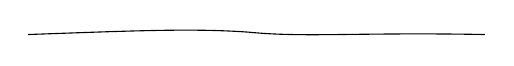
\begin{tikzpicture}
\draw (0,0) .. controls (1.4,.05) and (2.1,.08) .. (2.8,.03)
.. controls (3.5,-.04) and (4.2,.03) .. (5.8,0);
\end{tikzpicture}}

\textcircled{c}\quad We have
\[
(13)\qquad
N_\rho^*=\left\{u\in\mathcal M\mid u(\rho)=\rho^{\varepsilon_3(u)}\right\}
\quad\inserted{\bigl(=\varepsilon_3[\tau'](\rho)\bigr)}
\]

and
\[
(14)\qquad
\left\{\begin{aligned}
N_\rho^*\cap\widehat{\mathcal G}
  &=\mathbb D_\rho=\{1,\tau'\}.L_\rho\\
N_\rho^*\cap\mathcal G
  &=L_\rho\qquad(\simeq\mathbb Z/6\mathbb Z)\\
N_\rho^*\cap\Pi&=\mu\\
N_\rho^*\cap\Pi_0&=\{1\}
\end{aligned}\right.\qquad .
\]

\scanpage{624}

Let
\[
(15)\qquad
N_{\rho0}^{*!}\overset{\mathrm{dfn}}=N_\rho^*\cap\mathcal M_0^!,
\qquad N_\rho^{*!}=N_\rho^*\cap\mathcal M^!.
\]

we find
\[
(16)\qquad
N_{\rho0}^{*!}\subset Z_\rho
=\operatorname{Cent}_{\unsure{\mathcal M(0)|\mathcal M}}(\rho)
=\operatorname{Cent}_{\mathcal M}(L_\rho)
\]

and we also note
\[
(17)\qquad N_{\rho,0}^{*!}=Z_{\rho0}^{!}=\mathcal M'(-\bar j).
\]

We see that the homomorphism $\mathcal M\to\gamma_{\rho,\sigma}
=\widetilde{\Gamma}_{\mathbb Q}$ induces an \uline{isomorphism}

\( (\unsure{18}) \)\quad
\diagram{\begin{tikzcd}[column sep=large,row sep=small]
\mathcal M'(-\bar j)=Z_{\rho,0}^{!} \arrow[r,"\sim"] &
\gamma'_{\rho,\sigma}=\widetilde{\Gamma}_{\mathbb Q}
\arrow[d,phantom,"{\rotatebox{90}{$=$}\ \mathrm{dfn}}"]\\
&\{\gamma\in\gamma_{\rho,\sigma}\mid\varepsilon_3(\gamma)=1\}
\end{tikzcd}}

from which we deduce splittings into semidirect products
(or even direct products)
\[
(19)\qquad
\left\{\begin{aligned}
\mathcal M'&\simeq\mathcal M'(-\bar j).\mathcal G^{+\wedge}\\
\mathcal M^{\prime!}&\simeq\mathcal M'(-\bar j).\Pi\\
\mathcal M_0^{\prime!}&\simeq\mathcal M'(-\bar j).\Pi_0\\
Z_\rho^!\unsure{=|\simeq}\unsure{N_\rho^{*!}}
  &\simeq\mathcal M'(-j)\times\mu\\
\deleted{\unsure{N_\rho^*}}Z_\rho
  &\simeq\mathcal M'(-j)\times L_\rho
\end{aligned}\right.\qquad .
\]

\deleted{The correspondence between}
\diagram{\begin{tikzcd}[nodes in empty cells]
\deleted{\unsure{\mathcal M^{!\prime}[0]|\mathcal M^{\prime!}[0]}}
\arrow[r,"{\deleted{\sim}}"] & \deleted{\gamma'_{\rho,\sigma}}
\end{tikzcd}}
\deleted{and}
\diagram{\begin{tikzcd}[column sep=small,nodes in empty cells]
\deleted{\mathcal M(-j)} \arrow[r,phantom,"{\deleted{\subset}}"]
\arrow[rr,bend right=25,"{\deleted{\sim}}"'] &
\deleted{N_\rho^*} & \deleted{\gamma_{\rho,\sigma}}
\end{tikzcd}}
\deleted{is defined by the map}

\deleted{\( (18) \)}\quad
\diagram{\begin{tikzcd}[nodes in empty cells]
\deleted{\unsure{\mathcal M^{!\prime}[0]|\mathcal M^{\prime!}[0]}}
\arrow[r] & {}
\end{tikzcd}}
